The \texttt{export} package provides the classes used by the application to transform given \texttt{\hyperref[type:edu.kit.wavelength.client.model.term.LambdaTerm]{LambdaTerms}} into a String representation depending on the selected format. Also the \texttt{export} package contains a \texttt{\lnk{Exports}} class that provides information about the available export formats. 

All format classes implement the interface \texttt{\lnk{Export}}. The representation of a given \texttt{\hyperref[type:edu.kit.wavelength.client.model.term.LambdaTerm]{LambdaTerm}} can thus be requested via a unique method. 
The second method of the interface returns the name of the export format to the caller.
Since these classes just transform the given terms, it is not guaranteed that the generated representation is executable. This concerns mainly the classes \texttt{\lnk{HaskellExport}} and \texttt{\lnk{LispExport}}.

All available export formats can be requested by calling the \texttt{\lnk{Exports}} class. Its single method returns a collection of the export format classes.  

\begin{figure}[H]
	\centering
	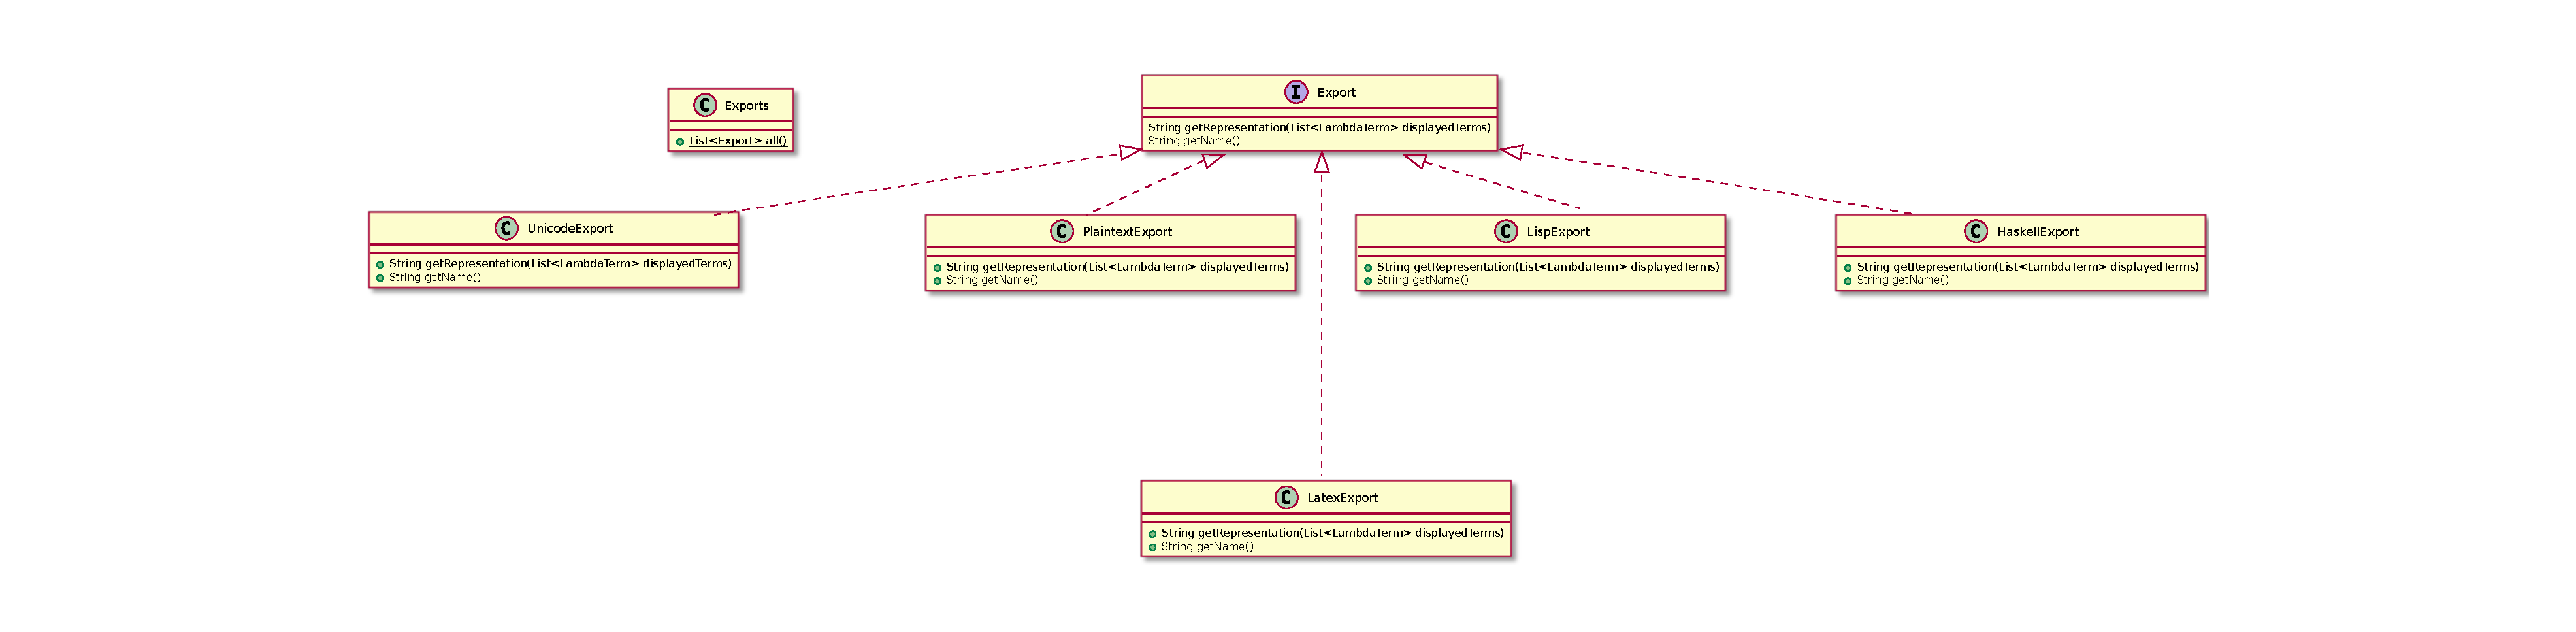
\includegraphics[width=\textwidth]{packageDiagrams/exportPackage}
\end{figure}
